\subsection{RQ3: Relation between the advancement of new languages and its developers' activity}
\label{RQ3}
Being the most used QA site Stack Overflow provides us an insight into the developers' activity pattern. \textcolor{green}{The most common developers' activities in SO \citep{Badashian2014} are,
\begin{enumerate}
    \item \textbf{Questions:} Developers ask development-related questions. Questions might be moderated based on clarity and duplicity.
    \item \textbf{Answers:}  Developers answer questions about their field of expertise.
    \item \textbf{Comment:} Users can comment on other users' questions and answers.
    \item \textbf{Up Votes:} Developers can vote to increase the score of other users' questions or answers.
    \item \textbf{Down Votes:} Developers can cast votes to decrease the score of other users' questions or answers.
    \item \textbf{Question View:} Users can view other users' questions. ( SO does not keep this count with a timestamp).
    \item \textbf{Answer View:} Users can view other users' answers. ( SO does not keep this count with a timestamp).
\end{enumerate}}
We can get the activity pattern of the developers' of a new programming language from the question-answer frequency of that language. High developers' activity helps to expose special cases and rare bugs of a project. Developers use the issue to inform the language owners about these problems or a particular case. The solution to these problems and bugs led to the growth of the language. Hence, we expect a  relationship between issue and developer's activity pattern. Moreover, developers' activity can also be observed from the number of users, repositories of that language from GitHub. \textcolor{green}{Table ~\ref{table:model parameters} summarizes the descriptions of and rationales behind the studied factors.} To measure the relationship among variables we have performed the following steps.
\begin{table}[]
\begin{tabular}{lll}
\hline
Factor name                & Description & Rationale \\ \hline

Number of questions posted &             &           \\ \hline

Open Issue Count           & \begin{tabular}[c]{@{}l@{}}The number of open \\issue in the official\\ repository of that\\ language\end{tabular}           &    \begin{tabular}[c]{@{}l@{}}This factor reflects\\the maturity of\\language\end{tabular}       \\ 

Closed Issue Count         &   \begin{tabular}[c]{@{}l@{}}The number of closed \\issue in the official\\ repository of that\\ language\end{tabular}          &    \begin{tabular}[c]{@{}l@{}}This factor reflects\\the maturity of\\language\end{tabular}       \\ 

Ratio of Open Issue        & \begin{tabular}[c]{@{}l@{}}The ratio of the  open \\and closed issue in\\ the official repository\end{tabular}             &    \begin{tabular}[c]{@{}l@{}}This factor reflects\\the agility of\\the language project\end{tabular}        \\ \hline

Number of open issue       &             &           \\ \hline

User Count                 &  \begin{tabular}[c]{@{}l@{}}The number of new \\users of this language\\ on GitHub\end{tabular}            &   \begin{tabular}[c]{@{}l@{}}This factor reflects\\the effect of incomplete\\ release over the\\ reputation of the language\end{tabular}        \\ 

Repository Count           &  \begin{tabular}[c]{@{}l@{}}The number of new\\repositories of this\\language\\ on GitHub\end{tabular}        &     \begin{tabular}[c]{@{}l@{}}This factor reflects\\the effect of incomplete \\release over the\\ developer base\end{tabular}      \\ \hline
\end{tabular}
\caption{The description and rationale for the factors in the number of SO questions, and number of GitHub open issue.}
\label{table:model parameters}
\end{table}
\begin{enumerate}
    \item Model Construction (MC)
    \item Model Analysis (MA)
\end{enumerate}
These steps are discussed below.

\textbf{Model construction (MC):} 
We build a regression model to explain the relationship between dependent and explanatory variables. Regression model fits the dependent variable with respect to independent variables. We followed the model construction approach of Harrel et al.\citep{Harrell2015}. While relaxing the linearity assumption, this approach models the nonlinear relationship accurately.
The steps for model construction are described below.
\begin{enumerate}
    \item \emph{Estimation of maximum degrees of freedom:}
    A critical concern in model building is overfitting. Overfitting is most frequent in models that use more degree of freedom than the dataset can support. Hence, we have fixed the maximum degree of freedom for our model. As suggested by Harrel et al.\citep{Harrell2015}  we have fixed  \(\frac{n}{15} \) degree of freedom for our model
    \item \emph{Normality adjustment:}
    We fit our regression models using the Ordinary Least Squares (OLS) technique. OLS assumes the normality in the distribution of the dependent variable. Hence, it is crucial that the distribution of the dependent variable is normal. A widely used approach for conversion into a normal distribution is applying $\ln$ function\citep{pmid25092958}. We have some zero value in our dataset. Therefore in our case, we have used $\ln (x+1) $ to lessen the skew, and better fit the OLS assumption.
    \item \emph{Correlation analysis:}
    Before building the model, we checked the highly correlated explanatory variables. In this step, we have used Spearmen rank correlation as it is resilient to data which is not normally distributed. We have constructed a hierarchical overview of the correlation among explanatory variables. For sub-hierarchies of explanatory variables with correlation $\rho$ \textgreater 0.9, we selected only one element of the sub-hierarchy.
    \item \emph{Fit regression Model:}
    Finally, after selecting explanatory variables and log transformations of dependent variables, we fit our regression models to the data.
\end{enumerate}

\textbf{Model Analysis (MA):} 
We have calculated adjusted $R^2$ to measure the goodness of fit of the model. Adjusted $R^2$ takes into account the bias of additional degree of freedom by penalizing the model for each degree of freedom.
The steps for model analysis are described below.
\begin{enumerate}
    \item \emph{Assessment of Model stability:} 
    Adjusted $R^2$ may overestimate the performance of the model for the curse of overfitting. The performance estimation is taken into account by subtracting the average \emph{optimism}\citep{Efron1986}. The \emph{optimism} is calculated in three steps. First, a bootstrap is created from N samples. Second, a model is fitted on the bootstrap data using the same degree of freedom. Third, \emph{optimism}, the difference between the adjusted $R^2$ of the bootstrap model and the model built in the previous step(original model) is calculated. The process is repeated for 1000 times, and we have got average optimism. Finally, we subtracted the average optimism from original adjusted $R^2$ and got optimism reduced $R^2$.
    \item \emph{Estimation of the power of explanatory variables:}
    To measure the impact of an explanatory variable on a model, we measured the difference in performance between all explanatory variables(full model) and all explanatory variables except one(dropped model). A $\chi^2$ test is applied to the resulting values to detect whether each explanatory variable improves model performance to a statistically significant degree. To estimate the impact, we performed the Wald $\chi^2$ maximum likelihood test. The larger the Wald $\chi^2$ value, the more significant the impact of that particular explanatory variable is\citep{McIntosh2015}.

\end{enumerate}
We can observe the relation between developers' activity pattern and advancement of the language project from two different perspectives: (1) Question count of Stack Overflow and (2) Repository and User count of that language from GitHub. Hence, we performed the process of estimating the relationship for each perspective. We have used open issue count, closed issue count, and the ratio of open issue count with respect to the total number of the issue as the explanatory variable and the question count as the dependent variable to estimate the relationship between issue frequency and developers' activity from  Stack Overflow perspective. According to our methodology, results for the estimation of the relationship between the age and the developers' activity from the \textbf{perspective of Stack Overflow} is presented below.
\begin{table}
\centering

\caption{Coverage model statistics from the perspective of Stack Overflow}
\begin{threeparttable}
\begin{tabular}{|l|l|l|l|}
\hline
       & Swift & Go & Rust \\ \hline
    Adjusted $R^2$   &0.443  & 0.813 &0.924  \\ \hline
    Optimism-reduced $R^2$ & 0.441 &0.802  &0.919 \\ \hline
    Budgeted Degree of freedom & 8 & 8  &8 \\ \hline
%    Degree of freedom spent   & 3 & 4 & 3 \\ \hline
    Open Issue $\chi^2$             & 10 \tnote{*} & 53\tnote{**} & 10\tnote{*}\\ \hline
    Closed Issue $\chi^2$           & 59 \tnote{*}& 251\tnote{**} & 716\tnote{**} \\ \hline
    Ratio of Open Issue $\chi^2$    & 10 \tnote{*} & 63\tnote{**} & 21\tnote{**}\\ \hline
\end{tabular}


\begin{tablenotes}
\item [*] p\textless 0.1 
\item [**] p\textless 0.001
\end{tablenotes}
\end{threeparttable}
\label{table:issue_question relationship}
\end{table}



\begin{enumerate}[wide=0pt, leftmargin=*]
    \item[(MC-1)] \textbf{Estimation of the maximum degree of freedom:} We have 120  points in our dataset. Hence, by Harrel et al.\citep{Harrell2015} we can allow maximum 8 degrees of freedom.
    \item[(MC-2)] \textbf{Normality adjustment:} Question frequency of the new languages is right-skewed. So we have to perform log normality adjustment in this case.
    \item[(MC-3)] \textbf{Correlation analysis:}
    We hierarchically clustered the features by Spearmen $\mid \rho \mid$ value. It is found that the open issue ratio is highly correlated with closed issue count. For the sake of completeness, we have created a model using closed issue count instead of open issue ratio and vice-versa but have not found any change in the performance of the model.
    \item[(MA-1)] \textbf{Assessment of model stability:}
    Table~\ref{table:issue_question relationship} presents the adjusted $R^2$ and optimism corrected $R^2$. From Table~\ref{table:issue_question relationship}, we can say that the model is stable for Swift and Go where the optimism (the difference between Adjusted $R^2$ and Optimism-reduced $R^2$) is 0.002 and 0.005 respectively. However, for Go, the optimism is 0.011. Though the difference is noteworthy, it does not invalidate our model.
    \item[(MA-2)] \textbf{Estimation of the power of explanatory variables:}
    The high $\chi^2$ value of the open issue and the ratio of the open issue to the total number of issue in  Table~\ref{table:issue_question relationship} represents the significant role of these parameters in Stack Overflow. However, they are not that much significant for determining the number of Swift and Rust language questions in Stack Overflow. On the other hand, closed issue ratio is significant for all three languages in determining the number of questions in Stack Overflow which is proved by the high $\chi^2$  value of closed issue in Table~\ref{table:issue_question relationship}. Overall,  the $\chi^2$ value of Swift language is relatively smaller than the other two languages. Hence, we can say that the GitHub issue provides a meaningful and robust amount of explanatory power in describing question frequency of new languages except Swift.
\end{enumerate}
It is quite clear from the adjusted $R^2$ value of Table~\ref{table:issue_question relationship} that there is a relationship between language the growth of a language and the number of questions posted. As seen from Table~\ref{table:issue_question relationship}, the number of closed issues is the most impactful explanatory variable for the Rust language model. Hence, we can say that the number of open issues will significantly influence the number of Rust question in Stack Overflow.
Developers use an issue to ask owners about a new feature and seeking help about any problems. More developers may lead to a high number of issues. Therefore, from GitHub perspective, to model a relationship between issue and the developers' activity we have used User count of that language and Repository count of that language as the explanatory variable and Open issue count as the dependent variable. The relationship between the growth of a language and the developers' activity from the perspective of GitHub is presented below.
\begin{table}
\centering
\caption{Coverage model statistics for relationship from the perspective of GitHub}
\begin{threeparttable}
\begin{tabular}{|l|l|l|l|}
\hline
       & Swift & Go & Rust \\ \hline
    Adjusted $R^2$   &0.755  & 0.907 &0.862 \\ \hline
    Optimism-reduced $R^2$ & 0.751 &0.905  &0.859 \\ \hline
    Budgeted Degree of freedom & 8 & 8  &8 \\ \hline
%    Degree of freedom spent   & 4 & 4 & 3 \\ \hline
    User $\chi^2$             & 64 \tnote{*} & 215\tnote{*} & 50\tnote{*}\\ \hline
    Repository $\chi^2$           & 289 \tnote{**}& 19\tnote{**} & 192\tnote{**} \\ \hline
\end{tabular}
\begin{tablenotes}
\item [*] p\textless 0.1 
\item [**] p\textless 0.001
\end{tablenotes}


\end{threeparttable}
\label{table:github_question relationship}
\end{table}



\begin{enumerate}[wide=0pt, leftmargin=*]
    \item[(MC-1)] \textbf{Estimation of the maximum degree of freedom:}  To answer this question we have used the same dataset used in the previous step. Hence, we can allow a maximum of 8 degrees of freedom.
    \item[(MC-2)] \textbf{Normality adjustment:} Like the previous step, we have applied a log transform to normalize the dependent variable(open issue count).
    \item[(MC-3)] \textbf{Correlation analysis:}
    We have used two feature to build this model. Hence, instead of hierarchical clustering, we just calculated the Spearmen $\mid \rho \mid$ value between \emph{user count} and \emph{repository count}. It is found that they are not correlated.
    \item[(MA-1)] \textbf{Assessment of model stability:}
    Table~\ref{table:github_question relationship} presents the adjusted $R^2$ and optimism reduced $R^2$. From Table~\ref{table:github_question relationship} the optimism for each language is \textless 0.01 which ensures the stability of the model.
    \item[(MA-2)] \textbf{Estimation of the power of explanatory variables:}
    The issue is associated with the developers' experience. Hence, we expect `User' parameter to be an important feature in determining the number of open issue in the official GitHub repository of new languages. Table~\ref{table:github_question relationship} shows a high $\chi^2$ value of user count parameter, which supports our conjecture about the significance of the number of users in determining the number of open issue in GitHub. We have also found that Rust has relatively less user in GitHub compared to the other two languages which are expressed in the $\chi^2$ value of `User' parameter for Rust. The high $\chi^2$ value of the repository parameter for Swift and Rust language represents the significance of the number of the repository in determining the number of Swift and Rust open issue. However, the number of repositories is less significant in determining the number of open issue in the Go GitHub repository compared to the other two languages.
\end{enumerate}
From the adjusted $R^2$ value of Table~\ref{table:github_question relationship}, it is clear that there is a strong relationship between developers' GitHub activity and the number of open issue in the official repository of that respective language. 

\boxtext{\textbf{Finding 4:} There is a relationship between developers' activity pattern and the growth of the language.}

\boxtext{\textbf{Finding 5:} The number of open issues of Rust in GitHub significantly influenced the number of questions on Rust in Stack Overflow.}

\boxtext{\textbf{Finding 6:} The open issue count of Swift and Rust is highly dependent on the number of repositories of that language in GitHub.}


Every new release impacts the growth of a programming language. The developers' activity after a new release can give us an idea about the relationship between developers' activity pattern and the growth of a language. To observe the developers' activity pattern after a new release, we have collected all release dates of new languages from GitHub and then plotted them alongside question, issue, and repository count.

\begin{figure}[h]
 \centering
\begin{subfigure}{0.6\textwidth}
\hspace{40pt}
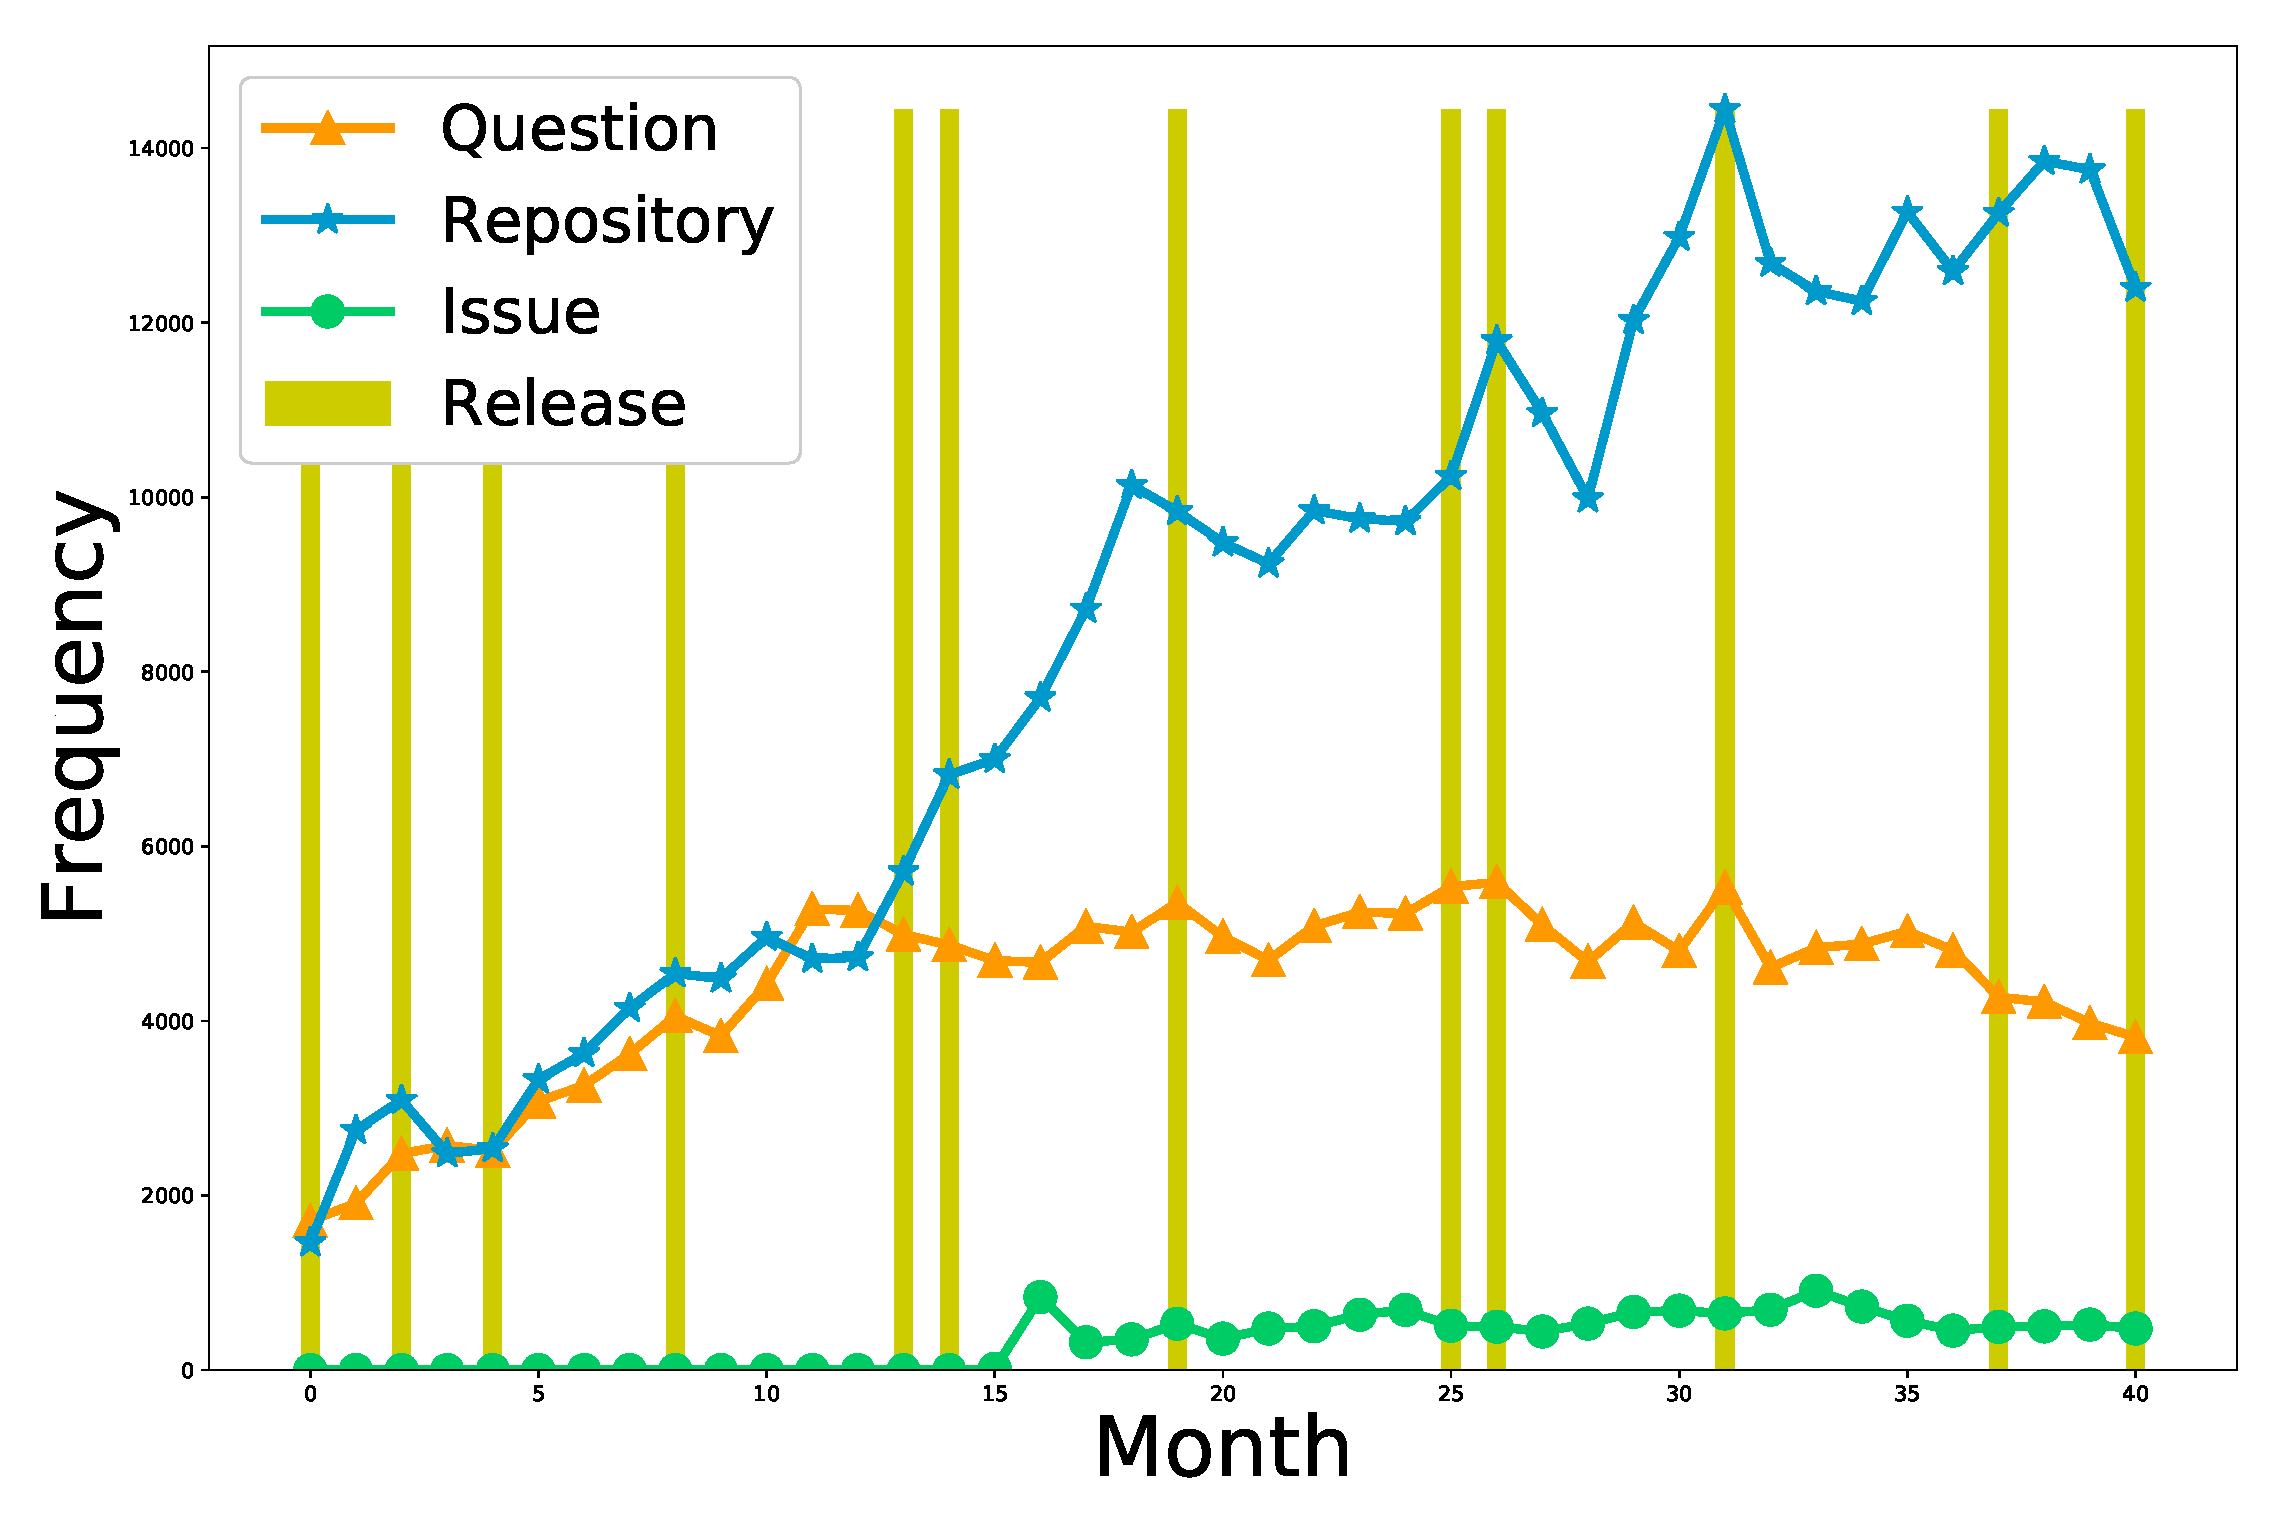
\includegraphics[scale=0.14]{figures/Swift_release_and_user_behaviour} 
\caption{Swift language}
\label{fig:Question count for Swift}
\end{subfigure}
\begin{subfigure}{0.6\textwidth}
\hspace{40pt}
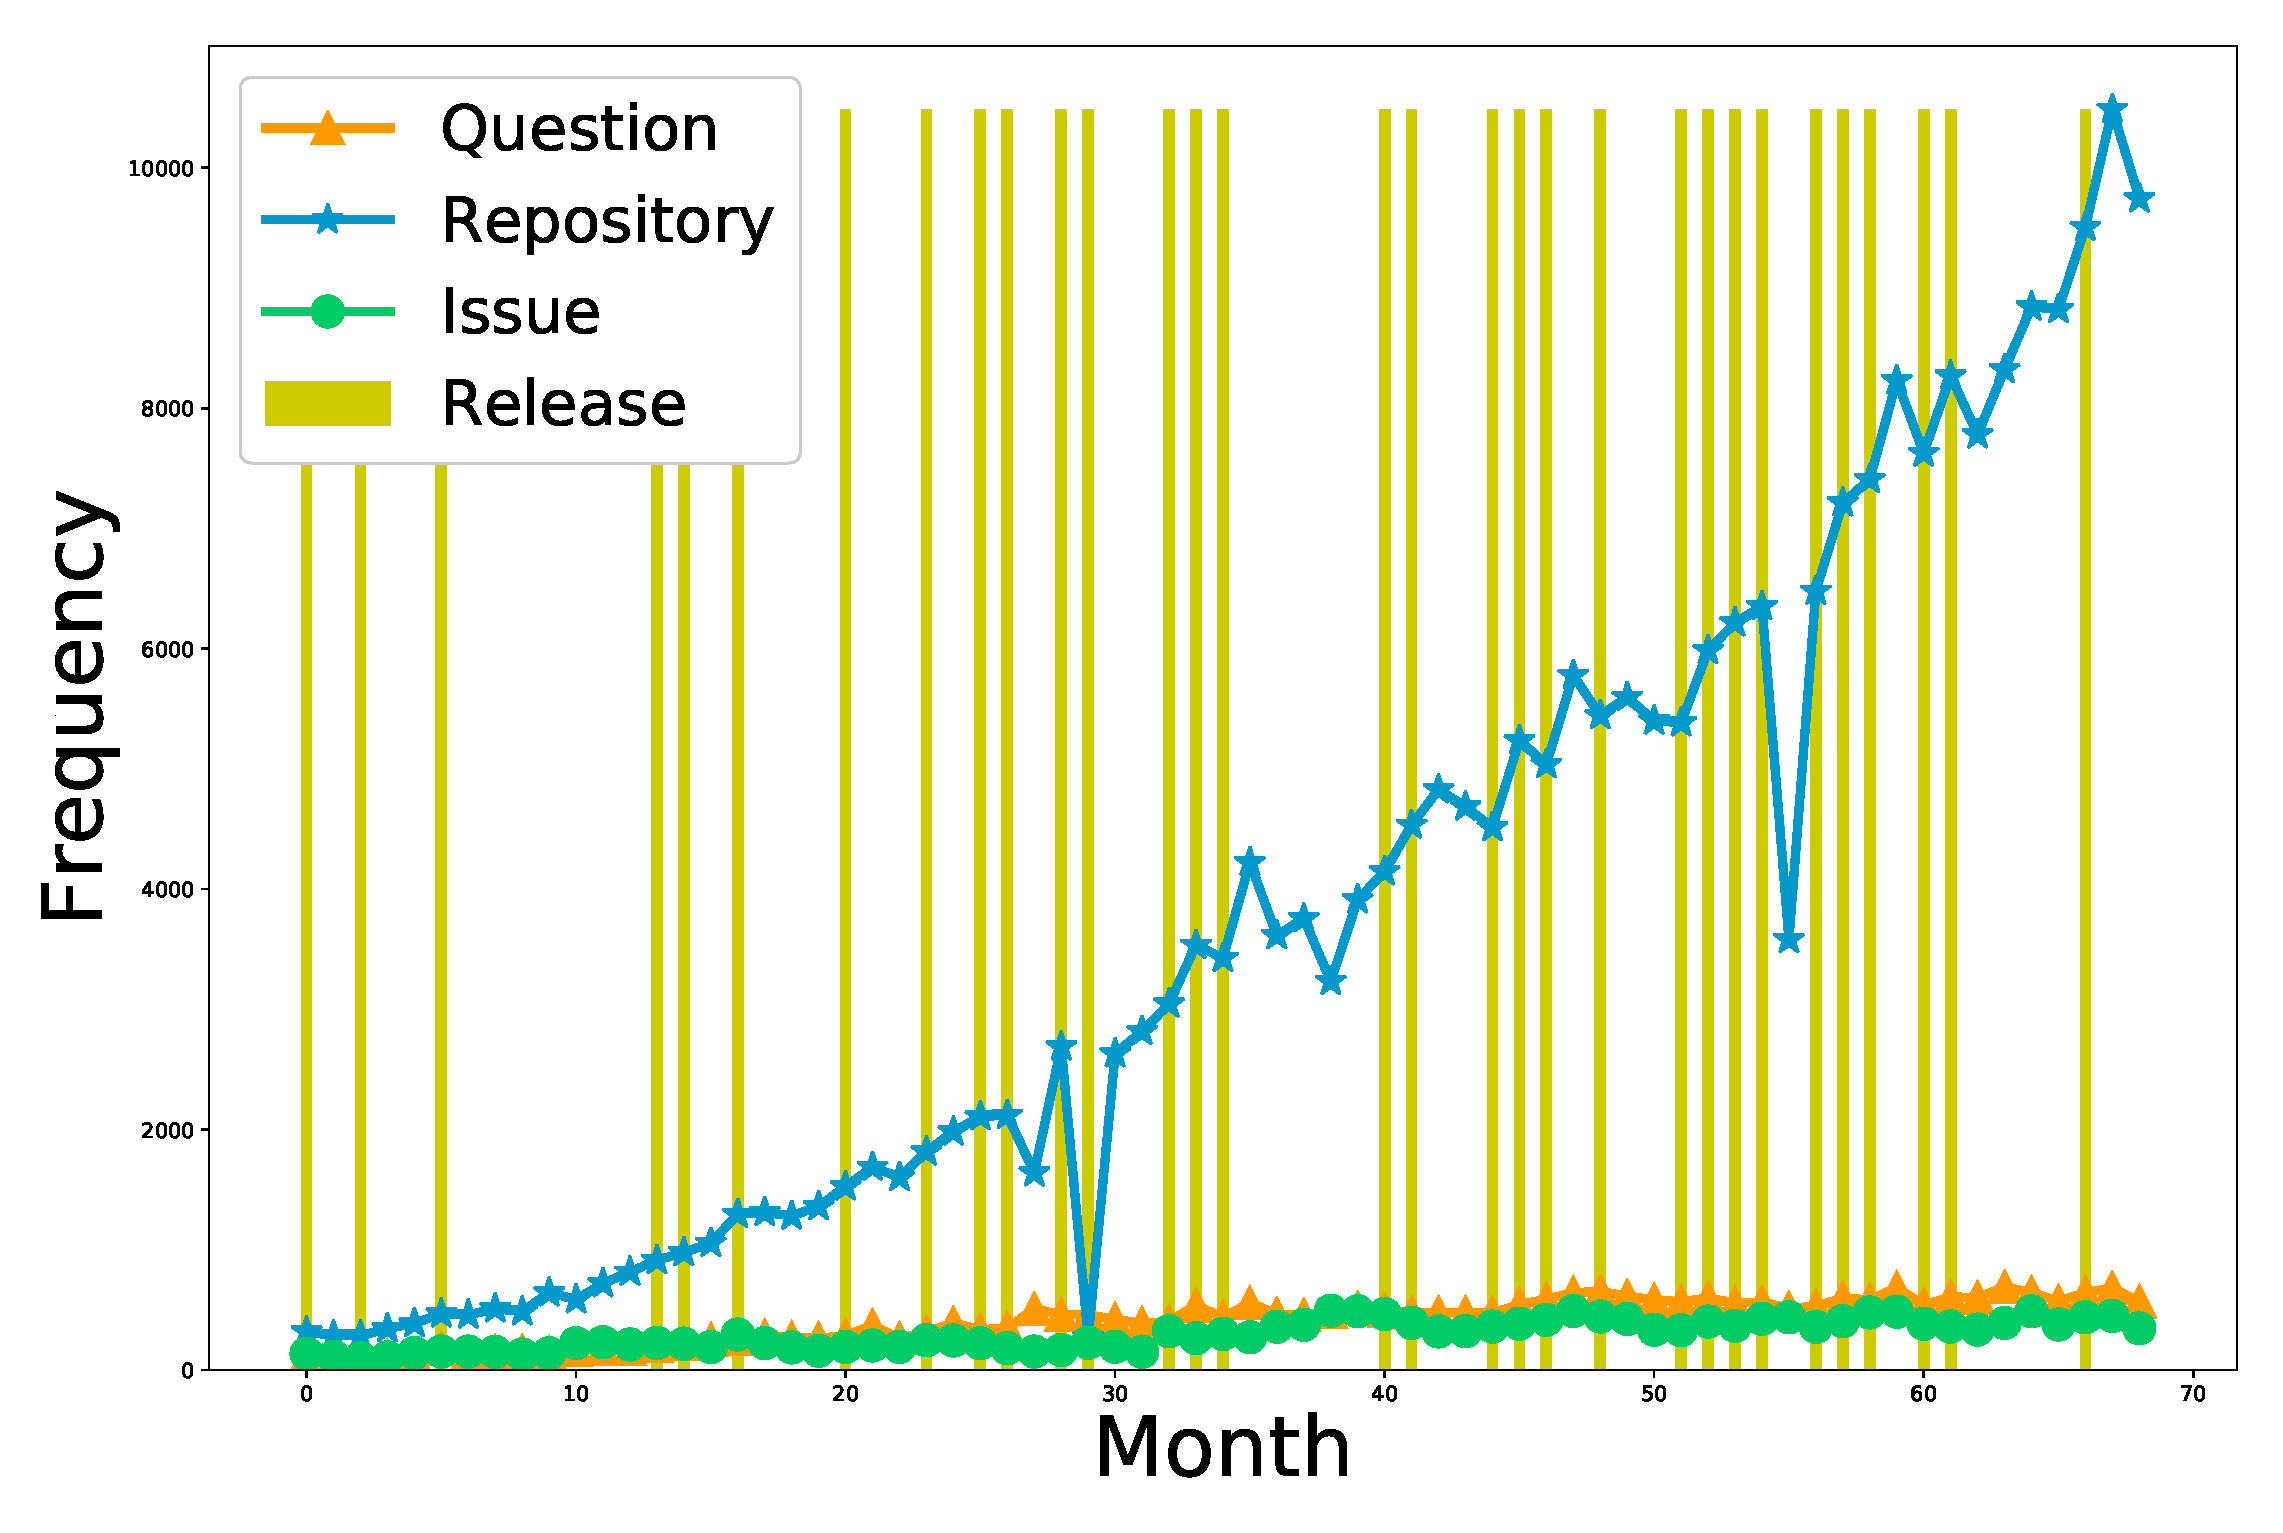
\includegraphics[scale=0.14]{figures/Go_release_and_user_behaviour}
\caption{Go language}
\label{fig:Question count for Go}
\end{subfigure}
\begin{subfigure}{0.6\textwidth}
\hspace{40pt}
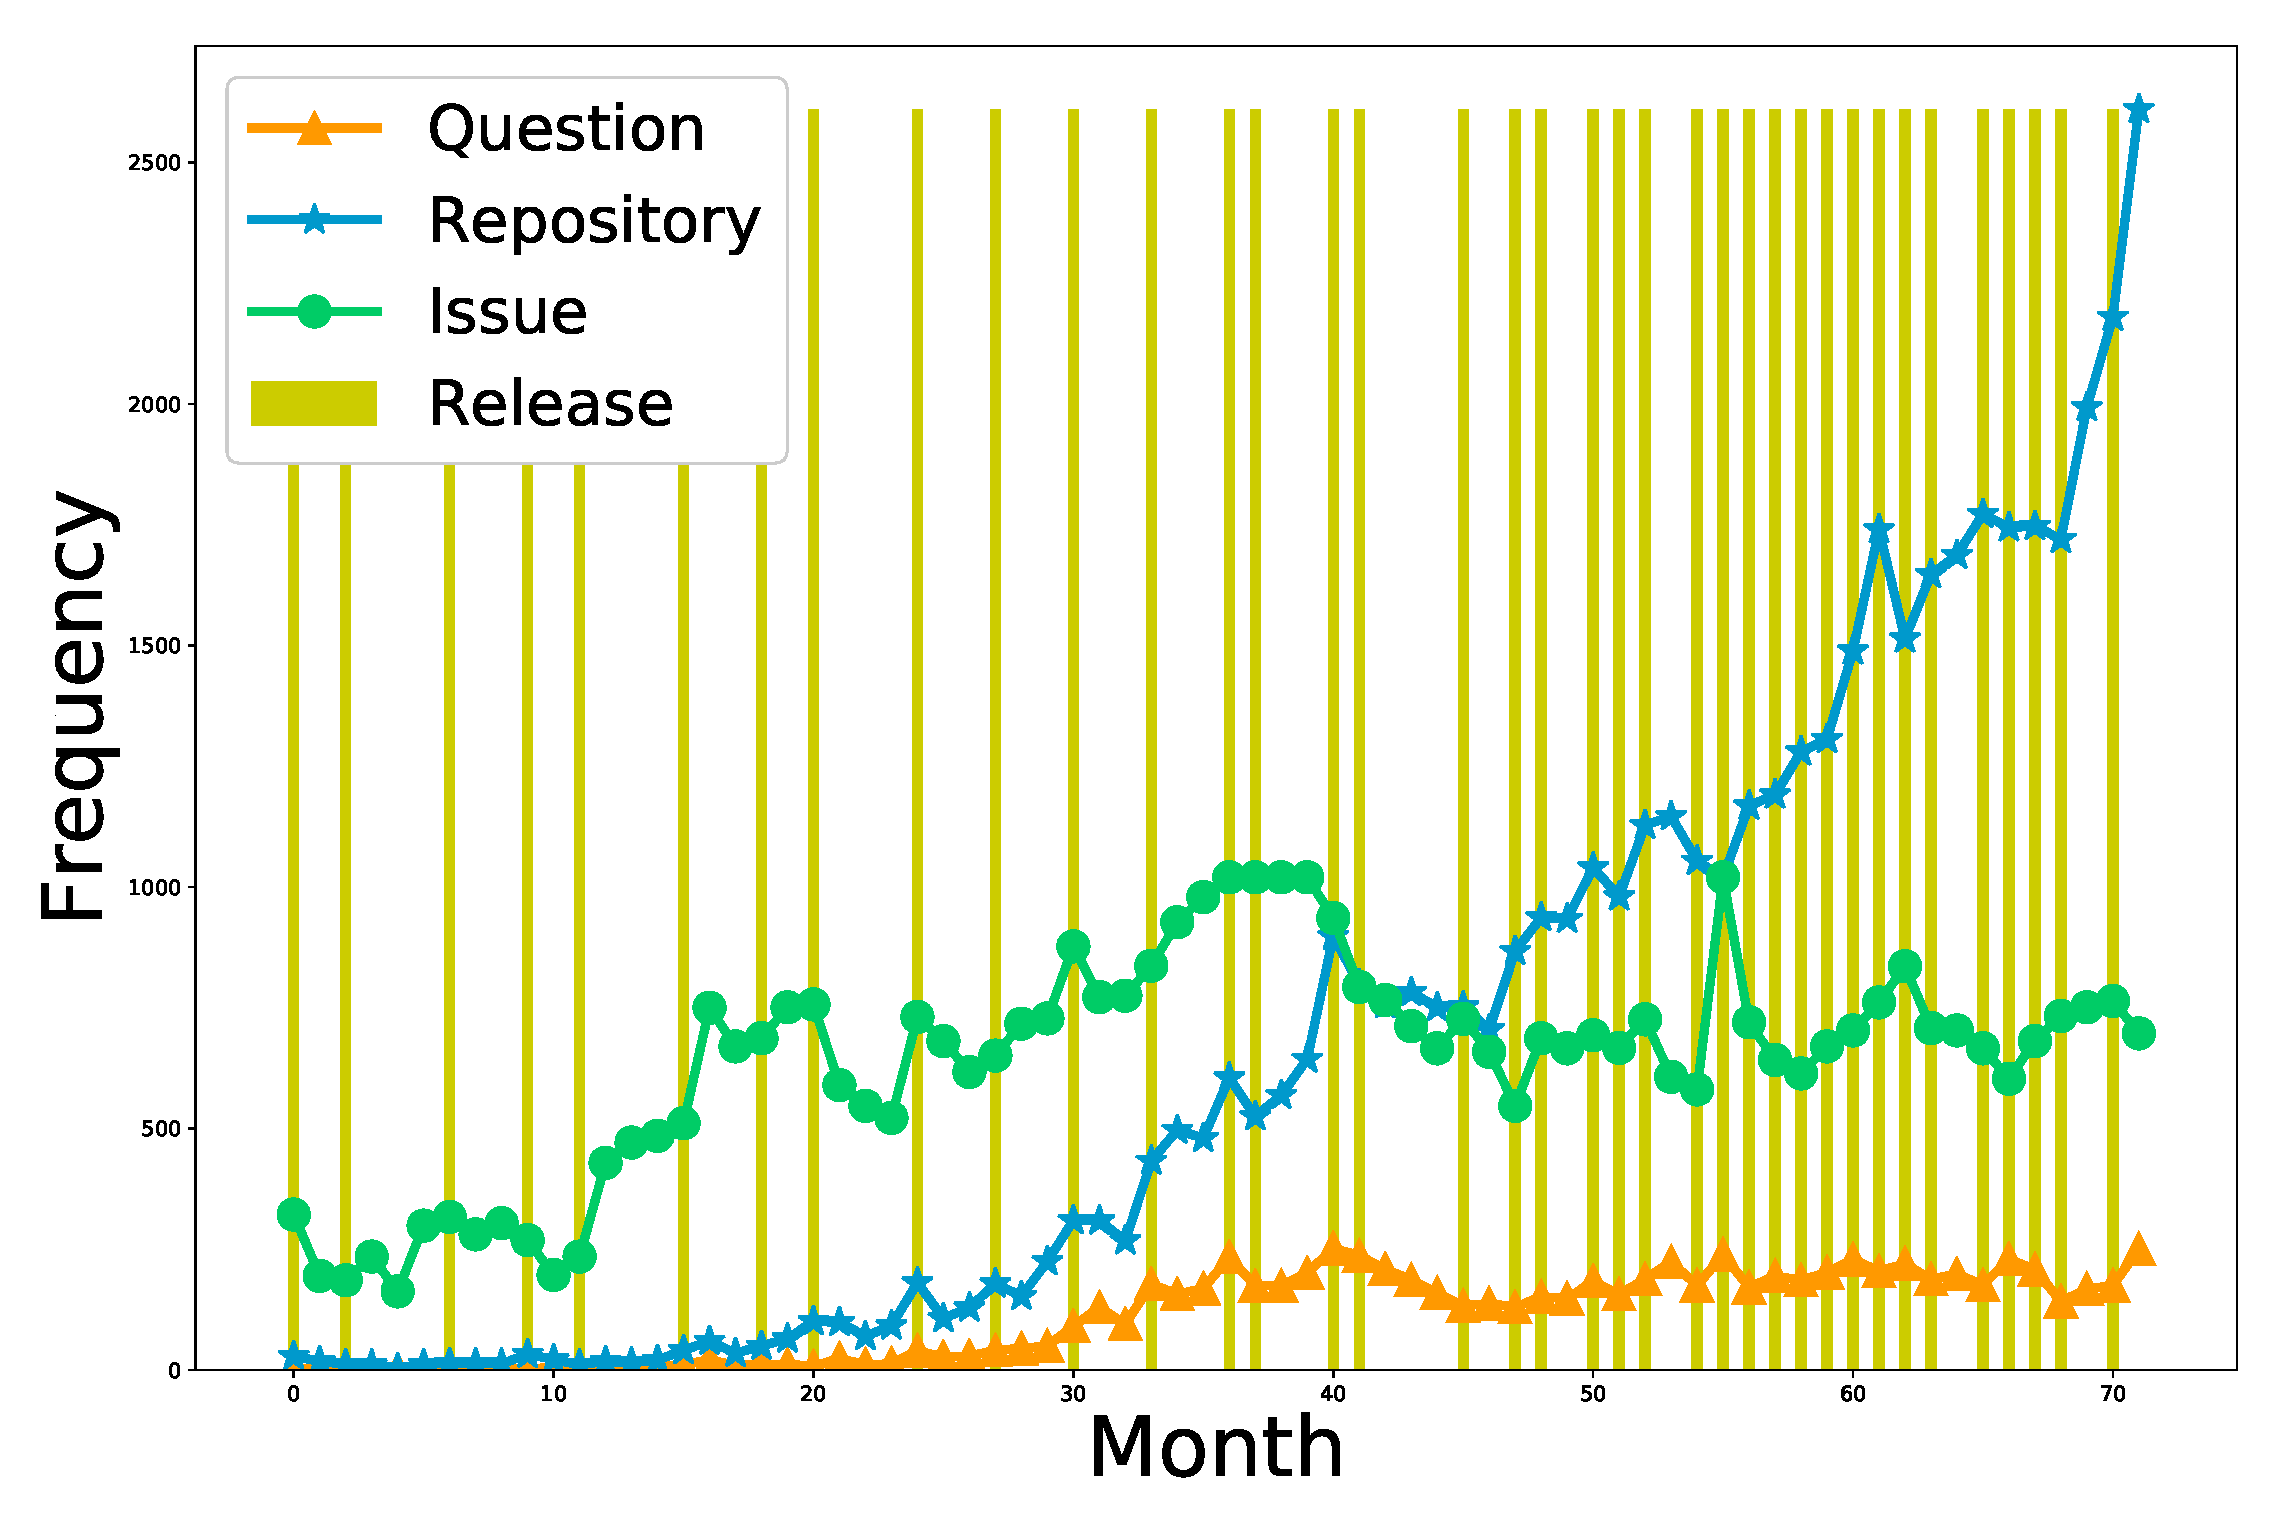
\includegraphics[scale=0.14]{figures/Rust_release_and_user_behaviour}
\caption{Rust language}
\label{fig:Question count for Rust}
\end{subfigure}
\caption{Release of a new version and activity pattern of the developers of respective languages}
\label{fig:Release and user behavior}
\end{figure}
Each sub-figure shows the response after the release of a new version. That means developers' activity is influenced by the benefits, features, and bugs of the new release. This trend is also visible  in question count i.e., question count increases after each release (Figure~\ref{fig:Release and user behavior}). However, we observed that issue count of Swift is less influenced than that of the other two languages. For tracking bugs and language problem,  Go\footnote{https://Golang.org/project/} and Rust\footnote{https://github.com/Rust-lang/Rust/blob/master/CONTRIBUTING.md} use only GitHub issue tracker. On the other hands, besides using GitHub issue tracker, Swift\footnote{https://Swift.org/contributing/\#reporting-bugs} uses their own JIRA\citep{wiki:JIRA} instance for tracking bug\footnote{https://bugreport.apple.com/}. This is a likely cause of the difference, and as a result, the issue count of Swift represents a portion of the actual issue(bugs), and so it is less influenced by a new release than the other two languages. We have tested this hypothesis using statistical testing. We have performed Wilcoxon signed-rank test between the question, repository and issue count of the month before release and the count of the month of release. The result is presented in Table~\ref{table:release_impact}. However, only the change in repository count was significant. The reason behind significance is after each new release developers create a new repository to test the new features without altering the production version of the software. Hence, the number of repository increases after a new release. Though we can observe that the question and issue count 
\begin{table}
\centering
\caption{Wilcoxon signed rank test result for the comparison of change between before and after of a release.}
\begin{tabular}{|c|c|c|c|}
\hline
\multicolumn{1}{|l|}{Language} & \begin{tabular}[c]{@{}c@{}}Question\\ p value\end{tabular} & \begin{tabular}[c]{@{}c@{}}Repository\\ p value\end{tabular} & \begin{tabular}[c]{@{}c@{}}Issue\\ p value\end{tabular} \\ \hline
Swift                          & 0.583                                                      & \textless{}0.01                                              & 0.6                                                     \\ \hline
Go                             & 0.149                                                      & \textless{}0.01                                              & 0.433                                                   \\ \hline
Rust                           & 0.473                                                      & \textless{}0.01                                              & 0.2                                                     \\ \hline
\end{tabular}
\label{table:release_impact}
\end{table} are responding with the release of a new version, it is statistically insignificant according to the Wilcoxon signed-rank test. To find the reason behind this insignificance, we conducted a further investigation. We noticed that the spikes in question and issue count curve does not appear immediately after a release. Rather, it appears after a variable time gap. Thus, the change in question and issue count is statistically insignificant.


